\chapter{Transformations of {HTN} {M}odels}

\medskip\noindent
After an enumeration of various definitions and semantics, we will finally start discussing the transformation of different HTN models. This chapter will exhibit varying transformations along divergent contexts and preconditions. For example, HTN models might be partially-ordered, totally-ordered, with or without \emph{goal tasks}, having a different set of allowed \emph{state-constraints}.

\section{Normal Forms}

\medskip\noindent
The first section of this chapter is inspired by the \emph{Chomsky normal form} (CNF)~\cite{chytil}. A context-free grammar (\emph{CFG}) is in CNF if all of its production rules are of the form: $A \rightarrow BC$, $A \rightarrow a$, $S \rightarrow \varepsilon$ (in this case $S$ cannot be on the right side of a production rule) where $A, B, C$ are nonterminal symbols, $a$ is a terminal symbol, $S$ is a starting nonterminal symbol, and $\varepsilon$ denotes an empty symbol. This "nice" form of CF grammar allows us to prove important theorems about CF languages more easily. Similarly, we want to have "nice" forms of \emph{planning domains} without \emph{empty methods} which might speed up algorithms for planning, or plan verification. Also, these forms are useful for proving HTN theorems~\cite{langclassification}~\cite{cmyk}.

\begin{defn}\label{def04:14} \cite{langclassification}
    A \emph{hierarchical planning problem} $\mathcal{P} = (s_0,\omega,\mathcal{D})$ is said to be in $\text{NF}_{\geq 2}$ if all methods are of the form: $T \rightarrow T_1, \dots, T_k \; [C], k \geq 2$; $T \rightarrow a \; [C]$ where $T, T_1, \dots, T_k$ are \emph{compound tasks}, and $a$ is a \emph{primitive task (action)}.
\end{defn}

\begin{defn}\label{def04:15}
    A \emph{hierarchical planning problem} $\mathcal{P} = (s_0,\omega,\mathcal{D})$ is said to be in \emph{HTN-CNF} if all of its methods are of the form: $T \rightarrow T_1, T_2 \; [C]$; $T \rightarrow a \; [C]$ where $T, T_1, T_2$ are \emph{compound tasks}, and $a$ is a \emph{primitive task}. 
\end{defn}

\medskip\noindent
In Definitions~\ref{def04:14},~\ref{def04:15} we exclude the possibility of having empty \emph{plans} but this decision can be interchanged at any time. Moreover, these definitions do not allow \emph{empty methods}.

\begin{defn}\label{def04:16}
    We say that two \emph{planning problems} $\mathcal{P'}$, $\mathcal{P''}$ are equivalent if the set of solutions of $\mathcal{P'}$ is equal to the set of solutions of $\mathcal{P''}$.
\end{defn}

\begin{defn}\label{def04:17}
    \emph{A method} $T \rightarrow T_1, \dots, T_k \; [C]$ has \emph{linear ordering-constraints} $C$ if $subtasks$ can be split into disjunctive sets (set partition) $S_1, \dots, S_k, k \geq 1$ such that all \emph{ordering-constraints} between tasks are within the same set, and all tasks within one set $S_i$ are linearly ordered (if any two tasks aren't comparable within a set directly then we apply a transitive closure). Tasks not contained in any of \emph{ordering-constraints} are in sets of one element.
\end{defn}

\begin{defn}\label{def04:18}
    A \emph{hierarchical planning problem} $\mathcal{P} = (s_0,\omega,\mathcal{D})$ is said to be in \emph{HTN-GNF~\cite{gnf}} if it is TO and all of its methods are of the form: $T \rightarrow a, T_1, T_2, \dots, T_i \; [C], \; i \geq 0$; where $T, T_i$ are \emph{compound tasks}, and $a$ is a \emph{primitive task}. 
\end{defn}

\begin{thm}\label{thm04:5}
    Every \emph{planning problem} $\mathcal{P}$ (partially-, totally-ordered) that does not generate an empty \emph{plan} as a \emph{solution}, without \emph{state-constraints} (before, after, between) can be transformed into \emph{an equivalent planning problem} in $\text{NF}_{\geq 2}$.
\end{thm}
\begin{proof}
    The proof follows the ideas of the transformation of CFG into CNF~\cite{langclassification}. First of all, we need to get rid of \emph{empty methods}. For that, we need to find all \emph{nullable compound tasks}. \emph{A compound task} $T$ is \emph{nullable} if \emph{a method} $T \rightarrow \varepsilon \; [\{\}]$ exists, or if there is a sequence of \emph{decomposition} such that $T \rightarrow \dots \rightarrow \varepsilon \; [C]$. \emph{Nullable compound tasks} can be found followingly: for each \emph{method} $T \rightarrow \varepsilon \; [\{\}]$, $T$ is \emph{nullable}, and for each \emph{method} $T \rightarrow T_1, \dots, T_k \; [C], \; k \geq 1$ where $T_1, \dots, T_k$ are \emph{nullable}, $T$ is also \emph{nullable} (\emph{actions} are never \emph{nullable}). Having all \emph{nullable tasks}, we can remove \emph{empty methods} from the domain. After that, for each \emph{method} $T \rightarrow T_1, \dots, T_k \; [C]$ holding $i \geq 1$ \emph{nullable tasks} as subtasks, we create $2^i$ new methods with/without \emph{nullable tasks}, one special case is if $i = k$ then we do not create a new \emph{empty method} $T \rightarrow \varepsilon \; [C]$. All \emph{ordering-constraints} containing removed tasks are also removed in each new method. 
    
    The next step is to remove \emph{methods} of a form $T \rightarrow T_1 \; [\{\}]$ where $T, T_1$ are \emph{compound tasks}. These \emph{methods} will be called - \emph{unit methods}. For that, we need to find all \emph{unit pairs}. \emph{A unit pair} $(T_1, T_2)$ $T_1 \neq T_2$ is a pair of \emph{compound tasks} such that $T_2$ can be decomposed from $T_1$ only with the usage of \emph{unit methods}, i.e., $T_1 \rightarrow \dots \rightarrow T_2 \; [C]$. After that, for each \emph{unit pair} $(T_1, T_2)$ and for each non-\emph{unit-method} $T_2 \rightarrow T_i, \dots, T_j \; [C_2], i < j$, we create a new method: $T_1 \rightarrow T_i, \dots, T_j \; [C_2], i < j$ (\emph{ordering-constraints} are inherited from the second \emph{method}). Doing so, we can delete all \emph{unit-methods} from the \emph{planning problem} without the modification of \emph{solutions}.

    For each \emph{action} $a$ we produce a new \emph{compound task} $T_a$, a new \emph{method} $T_a \rightarrow a \; [\{\}]$, and for each \emph{method} $T \rightarrow T_1, \dots, T_k \; [C]$ having $a$ as a $subtask$ we delete $a$ from the $subtasks$ and include $T_a$ instead. All \emph{ordering-constraints} having $a$ are interchanged with ones containing $T_a$. 

    In this proof, we deleted all \emph{empty methods}, \emph{unit methods}, and modified \emph{methods} so they have single \emph{action} or \emph{compound tasks} as $subtasks$. Thus, all \emph{methods} left have a form: $T \rightarrow T_1, \dots, T_k \; [C], k \geq 2$; $T \rightarrow a \; [\{\}]$ where $T, T_1, \dots, T_k$ are \emph{compound tasks}, and $a$ is \emph{action}. In every step, we did not create nor remove any potential \emph{solution}.
\end{proof}

\begin{thm}\label{thm04:6}
    Every \emph{planning problem} $\mathcal{P}$ in $\text{NF}_{\geq 2}$, with all \emph{methods} containing only \emph{linear ordering-constraints}, without \emph{state-constraints} (before, after, between) can be transformed into \emph{an equivalent planning problem} in \emph{HTN-CNF}.
\end{thm}
\begin{proof}
     In this proof, we will need to divide the large \emph{methods} into smaller ones. Because all tasks are linearly ordered within the divided sets we know that there cannot be "ordering cycles", also we know that at every time in every task set, there is the first task, with respect to \emph{ordering-constraints}. A key feature of such constraints is that the tasks in sets are mutually independent because, from the definition, no \emph{ordering-constraints} exist between tasks from different sets. 

     Let us have \emph{a method} $T \rightarrow T_1, \dots, T_k \; [C], k \geq 3$, and a set partition of tasks $S_1, \dots, S_k, k \geq 1$ by the Definition~\ref{def04:17}. Now, we will transform the input \emph{planning problem} $\mathcal{P}$ into the result \emph{HTN-CNF} \emph{planning problem} in two steps. First, we will add new \emph{compound tasks} $S_1, \dots, S_k$ (same names as set partitions) and $k - 2$ $C_i$ \emph{compound tasks} to the \emph{planning problem}. After that, we will add new \emph{methods}: $T \rightarrow S_1, C_1 \; [\{\}]; \; C_1 \rightarrow S_2, C_2 \; [\{\}]; \; \dots; \; C_{k - 2} \rightarrow S_{k - 1}, S_k \; [\{\}]$. Newly created methods have an empty set of constraints because, as was mentioned, tasks from different partitions do not have any ordering relations between them. Therefore, their subtasks can interleave without any restrictions. 
     
     One special case that might occur is if the set of $subtasks$ is fully linearly ordered then there will be only one partition $S_1$. This situation can be handled easily. We will start the process of binarization right away. Similarly to the previous process, we will create $k - 2$ $X_i$ \emph{compound tasks}. After that, we will append new \emph{methods}: $T \rightarrow T_1, X_1 \; [\{T_1 \prec X_1\}]; \; X_1 \rightarrow T_2, X_2 \; [\{T_2 \prec X_2\}]; \; \dots; \; X_{k - 2} \rightarrow T_{k - 1}, T_k \; [\{T_{k - 1} \prec T_k\}]$ where $T_1$ is the first element with respect to \emph{ordering-constraints}, $T_2$ is the second element and so on.

     In the case of multiple sets $S_1, S_2, \dots$, we repeat the process above for each \emph{compound task} $S_i$ and for each partition $S_i$ independently. Doing so, we can delete the former \emph{method}. We iterate this process for all \emph{methods} with at least 3 tasks as subtasks.
\end{proof}

\begin{example}\label{ex04:7}
    If we want to binarize \emph{a planning domain} then we can use different types of \emph{ordering-constraints}. \emph{Method's} subtasks are binarizable if they can be split into two disjunctive sets of subtasks such that all subtasks in one set precede all subtasks in the second set, or if all subtasks in the first set have none \emph{order-constraints} with the second set of subtasks. \emph{A method} is binarizable if this process of splitting into two sets can be done repeatedly until all sets have a single task as an element. 
    
    Using graphs (\emph{DAG}) terminology where tasks are nodes and an arc $(a,b)$ exists if an \emph{order-constraint} $a \prec b$ exists, we can say that the graph can be split if it contains $\geq 2$ components, or a vertex $u$ exists such that in every topological sorting $u$ has the same position. If such a vertex exists then we know that all vertices with a higher number must come after $u$ and other vertices before. Thus we have 2 disjunctive sets of vertices and $u$ can be added to either of these two sets. A graph is binarizable if this process can be repeated until only single vertex is left.

    Figure~\ref{fig04:3} shows us the smallest \emph{DAG} that is not binarizable. Now we understand the reason for our choice of the \emph{linear ordering-constraints} in which we can always find the first or the last element.
    
    \begin{figure}
        \centering
        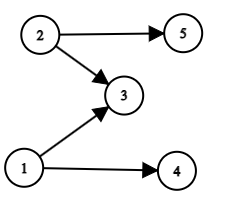
\includegraphics{img/graph.png}
        \caption{Unbinarizable graph}
        \label{fig04:3}
    \end{figure}
\end{example}

\begin{thm}\label{thm04:7}
    Theorem~\ref{thm04:5} transforms \emph{a planning problem} $\mathcal{P}$ with all \emph{methods} having \emph{linear ordering-constraints} into \emph{a planning problem} in $\text{NF}_{\geq 2}$ with all \emph{methods} having \emph{linear ordering-constraints}.
\end{thm}
\begin{proof}
    Theorem~\ref{thm04:5} includes two main parts: removing all \emph{empty methods} and \emph{unit-methods}. The elimination of \emph{unit-methods} does not have any effect on ordering because we need at least two tasks for \emph{an ordering-constraint}. We create new \emph{methods} without \emph{nullable} tasks which also deletes constraints containing these tasks. But because the ordering is linear even after the deletion of some elements (transitive closure from the definition) we do not create \emph{methods} that are not \emph{linear ordering-constraints}.
\end{proof}

\section{Totally-Ordered Transformations}

\medskip\noindent
Before we start with the transformation of \emph{totally-ordered planning problems} we need to tidy up \emph{state-constraints}. So far, \emph{state-constraints} are defined on sets of subtasks, i.e., $be\text{f}ore(p, U)$, $a\text{f}ter(U, p)$, $between(U, p, V)$ with $U, V$ denoting subsets of subtasks, and $p$ denotes \emph{a propositional symbol}. \emph{TO planning problems} allow us to remove unnecessary tasks from sets $U, V$ leaving us with only one subtask. Hence, we abuse the notation to let $be\text{f}ore(p, T)$ denote $be\text{f}ore(p, \{ T \})$ with $T$ being \emph{a method's} subtask. Similarly, we will use this notation for $a\text{f}ter$ and $between$ constraints. 

\begin{thm}\label{thm04:8}
    For each \emph{TO planning problem} there is \emph{an equivalent planning problem} with all \emph{state-constraints} operating with tasks instead of sets of sets of tasks.
\end{thm}
\begin{proof}
    Let us have \emph{a method} $T \rightarrow T_1, \dots, T_k \; [C], k \geq 1$, and a $be\text{f}ore(p, U) \in C$. This constraint can be transformed to $be\text{f}ore(p, T)$ such that $T \in U$ and $(\forall F \in (U - \{ T \})): T \prec F$. This can be done analogously for each $a\text{f}ter(U, p)$ and $between(U, p, V)$ constraint. If the result $between(U, p, V)$ constraint is of a form $between(T, p, F)$ and $F \prec T$ holds then this whole constraint can be removed from the set of constraints as there are none states to test this constraint. 
\end{proof}

\medskip\noindent
Now, all \emph{TO} domains will implicitly have only \emph{state-constraints} described in Theorem~\ref{thm04:8}.

\medskip\noindent\label{rem-between-two-tasks}
In the following parts, we will try to convert general \emph{TO planning problems} into ones of a \emph{HTN-CNF}. Initially, we will compile away $between$ constraints because this type of \emph{state-constraint} spans throughout states which is undesirable. This behavior complicates the conversion because the \emph{HTN-CNF} has at most two tasks as subtasks. In this case (\emph{HTN-CNF}), the $between(T_1, p, T_2)$ constraint is saying that the check is made before the application of the first \emph{action} to which $T_2$ decomposes, after the last \emph{action} to which $T_1$ decomposes, and also all states in between are checked. This means that the test is made in a single state after the last \emph{action} of $T_1$. This can be easily transformed to a single \emph{before-, after-constraint}. Complications with \emph{between-constraints} begin if we have at least three \emph{TO} subtasks $T_1 \prec T_2 \prec T_3$ and a $between(T_1, p, T_3)$ constraint. Having this, the check has to be made in (potentially) multiple states depending on a decomposition tree of \emph{a compound task} $T_2$. Transformation of this feature becomes difficult if we do not want to lose any information about \emph{a planning domain}.

\medskip\noindent
In~\cite{ondrckova2023semantics}~\cite{ondrckova2024empty} it is described how to get rid of $between$ constraints from \emph{TO planning problems} by adding a series of $be\text{f}ore$ constraints. This conversion is false as it does not concern all states between subtasks but only states before the first \emph{action} to which potential \emph{compound tasks} decompose. Compiling away $between$ constraints is more complicated but not impossible. The Algorithm~\ref{alg04:1} below shows how to do it properly.

\medskip\noindent
In the following Algorithm~\ref{alg04:1}, we will create new \emph{compound tasks} that are derived from the existing ones. Let us have \emph{a compound task} $T$. A new \emph{compound task} $T_{\{p, q\}}$ (same name but with a suffix) denotes that in every possible decomposition tree starting from $T_{\{p, q\}}$ all \emph{methods} do not contain any $between$ constraints, and every \emph{primitive task network} derived from the $T_{\{p, q\}}$ holds \emph{propositional symbols} $\{p, q\}$ in every state. These new \emph{compound task} will be replaced in \emph{methods} containing $between$ constraints, and as a result, it will allow us to remove these constraints. Also, we will use the notation $be\text{f}ore(Q, T)$ with $T$ being a task and $Q \subseteq P$ being a subset of \emph{propositional symbols}. $be\text{f}ore(Q, T)$ is just an abbreviation for a $be\text{f}ore(q_1, T), be\text{f}ore(q_2, T), \dots$ where $q_i \in Q$.

\begin{algorithm}
    \caption{TO into TO without between-constraints}\label{alg04:1}
    \begin{algorithmic}[1]
        \Procedure {Main}{\emph{TO planning problem}: $\mathcal{P} = (s_0,\omega,\mathcal{D})$}
            \State $NewCT \gets \{\}$ \Comment{New \emph{Compound Tasks}}
            \While {$\mathcal{D}$ contains \emph{a method} $m$ with \emph{a between-constraint}}            
                \For {each \emph{compound task} $t$ in $subtasks(m)$ that is part of $\geq 1$ \emph{between-constraints}}
                    \State $PropSymbols \gets \{p: between(T, p, F) \; and \; T \prec t \prec F \}$
                    \If {$T_{PropSymbols}$ not in $NewCT$}
                        \State find \emph{methods} $m'$ with $t = compound(m')$ and create new $M=(T_{PropSymbols}, subtasks(m'), constraints(m'))$
                    \EndIf
                    \State swap all occurrences of $t$ with $T_{PropSymbols}$ in \emph{a method} $m$
                \EndFor

                \For {each task $t$ in $subtasks(m)$}
                    \State $PropSymbols \gets \{p: between(T, p, F) \; and \; T \prec t \prec F \}$
                    \State \Comment{if $PropSymbols = \emptyset$ then constraints are always satisfied}
                    \State add $be\text{f}ore(PropSymbols, t)$, $a\text{f}ter(t, PropSymbols)$ to $m$
                \EndFor
                
                \State remove all \emph{between-constraints} from $constraints(m)$

                \For {each $T_{symbols}$ in $subtasks(m)$ ($T_{symbols}$ not in $NewCT$)}
                    \State $NewCT \gets NewCT \cup T_{symbols}$
                    \State SearchCompoundTask($T_{symbols}$)
                \EndFor
            \EndWhile
        \EndProcedure
        \Procedure {SearchCompoundTask}{\emph{Compound task}: $T_{InputSymbols}$}
            \For {each \emph{method} $m$ with $T_{InputSymbols} = compound(m)$}
                \For {each task $t$ in $subtasks(m)$}
                    \State $PropSymbols \gets \{p: between(T, p, F) \; and \; T \prec t \prec F \}$
                    \State add $be\text{f}ore(PropSymbols \cup InputSymbols, t)$ to $m$
                    \State add $a\text{f}ter(t, PropSymbols \cup InputSymbols)$ to $m$
                \EndFor

                \For {each \emph{compound task} $T$ in $subtasks(m)$}
                    \State $PropSymbols \gets \{p: between(K, p, L) \; and \; K \prec T \prec L \}$
                    \If {$T_{PropSymbols \cup InputSymbols}$ not in $NewCT$}
                        \State find \emph{methods} $m'$ with $T = compound(m')$ and create new $M=(T_{PropSymbols \cup InputSymbols}, subtasks(m'), constraints(m'))$
                    \EndIf
                    \State swap all occurrences of $T$ with $T_{PropSymbols \cup InputSymbols}$ in $m$
                \EndFor

                \State remove all \emph{between-constraints} from $constraints(m)$

                \For {each $T_{symbols}$ in $subtasks(m)$ ($T_{symbols}$ not in $NewCT$)}
                    \State $NewCT \gets NewCT \cup T_{symbols}$
                    \State SearchCompoundTask($T_{symbols}$)
                \EndFor
            \EndFor
        \EndProcedure
    \end{algorithmic}
\end{algorithm}

\begin{thm}\label{thm04:9}
    For each \emph{TO planning problem} there is \emph{an equivalent planning problem} without any \emph{between-constraint}.
\end{thm}
\begin{proof}
    First of all, we will compile away \emph{between-constraints} of the neighboring tasks, i.e., tasks $T_1 \prec T_2$ such that no task $T_i$ exist with $T_1 \prec T_i$ and $T_i \prec T_2$. As was said before, these constraints can be interchanged to a single \emph{before-constraint} ($between(T_1, p, T_2) = be\text{f}ore(p, T_2)$). \emph{Between-constraints} of a form $between(T_i, p, T_i)$ or $between(T_j, p, T_i)$ with $T_i \prec T_j$ are pointless and can be removed without any loss of information.
    
    The idea of the Algorithm~\ref{alg04:1} is to remove \emph{between-constraints} \emph{method} by \emph{method} with a procedure that might remind us of Depth-first search (DFS). Suppose a method \( M \) includes at least one \emph{between-constraint}. In every valid \emph{solution} of the \emph{planning problem} \(\mathcal{P}\) that employs \( M \) during the planning phase, there must exist a consecutive \emph{sub-plan} that is decomposed from the \( \text{compound}(M) \) and contains the \emph{propositional symbol} specified in the constraint.

    If we want to remove $between(T, p, F)$ constraint then we must ensure that all decompositions (even those with cycles) of all \emph{compound tasks} between $T$ and $F$ (with respect to \emph{TO}) hold \emph{propositional symbol} $p$.
    
    An algorithm is split into two distinct parts: the while-loop (3) in the \texttt{Main} function and a recursive function \texttt{SearchCompoundTask} (23). The main cycle removes all \emph{between-constraints} from a single \emph{method} per iteration meanwhile not creating any new \emph{between-constraints}. All \emph{compound tasks} that are mentioned in \emph{between-constraints} are substituted with new \emph{compound tasks} that are stored in an auxiliary set \texttt{NewCT} (2). If a substituted \emph{compound task} is already stored in \texttt{NewCT} then we do not have to recursively search this task with \texttt{SearchCompoundTask} function (17, 38). On the contrary, if the task is not searched then we need to create new \emph{methods} so that tasks from other \emph{methods} cannot be decomposed via \emph{methods} designed for the substituted tasks (7, 33).

    The recursive procedure \texttt{SearchCompoundTask} looks for all \emph{methods} that decompose the input \emph{compound tasks} and append constraints so that the \emph{propositional symbols} are checked in all states concerning the subtasks (27, 28). Also, the recursive procedure removes all \emph{between-constraints} during the search (35), so they are not found in the main while-loop.


    There is a finite number of \emph{propositional symbols}, \emph{methods}, \emph{compound tasks}, and new \emph{compound tasks} in \texttt{NewCT}. Therefore, the algorithm will not fall into an infinite cycle, and gradually all \emph{between-constraints} will be removed.
\end{proof}

\begin{thm}\label{thm04:10}
    For each \emph{TO planning problem} that does not generate empty \emph{plan} as a \emph{solution}, there is \emph{an equivalent planning problem} without \emph{empty methods}.
\end{thm}
\begin{proof}
    First, we will remove all \emph{between-constraints} with the Theorem~\ref{thm04:9}.

    Similarly to Theorem~\ref{thm04:5}, we will need to find all \emph{nullable tasks} in \emph{a planning problem} and create new \emph{methods} without these tasks. The difficult part is handling the \emph{before-, after-constraints} which need to be checked eventually. \emph{A nullable task} may have many different series of decompositions that lead to an empty set of tasks. Each of these decompositions may have different constraints that need to be checked. For this purpose, we will use a function $Nullifies(T)$ that accepts a \emph{nullable compound task} and returns a set of sets of \emph{propositional symbols}. Each element of the function's output represents one possible way of how we can decompose this \emph{compound task} and which \emph{propositional symbols} need to be checked.

    We will find all values of the function $Nullifies$ in the following inductive manner. \textbf{Base:} for each $T \rightarrow \varepsilon \; [\{\}]: Nullifies(T) = \{\{\}\}$. \textbf{Induction:} having $T \rightarrow T_1, \dots, T_k \; [C], \; k \geq 1$ with subtasks containing only \emph{nullable compound tasks} we extend $Nullifies(T) = Nullifies(T) \; \cup \; \{\{\text{propositional symbols mentioned in} \; C\} \\ \cup propSym_1 \cup \dots \cup propSym_k\}$ where $propSym_i \in Nullifies(T_i)$. The induction part is repeated until there is a new unique combination of \emph{propositional symbols} that is not mentioned in $Nullifies(T)$ with some \emph{nullable compound task} $T$ and some \emph{method} $T \rightarrow T_1, \dots, T_k \; [C], \; k \geq 1$.

    It can be easily seen that $T$ is \emph{nullable} if and only if $Nullifies(T) \neq \emptyset$ (after we have found all values). \emph{The compound task} in \emph{the initial task network} is never \emph{nullable} as stated in the theorem. This feature will be used in the second part of the \emph{empty method} elimination.

    At this point, all \emph{empty methods} can be removed from the \emph{planning domain}.

    Now, for the final part, we will append new \emph{methods} with/without \emph{nullable tasks} to the \emph{planning problem}, similarly to Theorem~\ref{thm04:5}. Suppose \emph{a method} contains $i$ \emph{nullable tasks} in $subtasks$. Without loss of generality, \emph{nullable tasks} will be $T_1, \dots, T_i$. There will be $(|Nullifies(T_1)| + 1) * \dots * (|Nullifies(T_i)| + 1)$ new \emph{methods}, some of them might be identical. For each such combination, we will create a new \emph{method} without (some) \emph{nullable tasks}. \emph{Ordering-constraints} mentioning deleted tasks are removed from the set of constraints. If we want to remove \emph{a nullable task} $T_j$ then we need to find the closest task that is not removed from the \emph{method} and shift \emph{state-constraints}. If the non-removed task $T_k$ holds $k < j$ then we create a new constraint: $a\text{f}ter(T_k, PropSymbols)$, $PropSymbols \in Nullifies(T_j)$. On the other hand, if $k > j$ then we append $be\text{f}ore(PropSymbols, T_k)$ to the set of \emph{method's} constraints. It might happen that all $subtasks(M)$ of \emph{a method} $M$ are \emph{nullable}, in this case, we do not create new \emph{empty method} because $compound(M)$ will be removed from \emph{methods} that contain $compound(M)$ as a subtask. As was stated before, \emph{initial task network} is never \emph{nullable}, thus we do not need to handle this awkward situation.
\end{proof}

\begin{thm}\label{thm04:11}
    For each \emph{TO planning problem} there is \emph{an equivalent planning problem} without any \emph{after-constraints}.
\end{thm}
\begin{proof}
    \emph{TO planning problems} allow us to shift any \emph{after-constraint} to the succeeding task. So, \emph{an after-constraint} is changed to \emph{before-constraint}. This transformation is valid with only one exception. If \emph{the after-constraint} targets the last task with respect to \emph{TO} then \emph{an after-constraint} cannot be shifted to the following task because such task does not exist in a set of \emph{method's} $subtasks$. One might think that we can compile this feature away using the cooperation with other \emph{methods}. Still, it can happen that the targeted task will be the last \emph{action} in \emph{the solution} which means that the check will be evaluated in a state after the execution of all \emph{actions} in \emph{the plan}. Therefore, in this case, we cannot shift \emph{an after-constraint} so easily. What we can do is to create a new \emph{compound task} $T_{empty}$ with one \emph{empty method}. Then, this task can be inserted at the end of \emph{a method} and problematic \emph{after-constraints} can be shifted to the $T_{empty}$.

    Symmetrically, we can transform all \emph{before-constraints} to the equivalent \emph{after-constraints}.
\end{proof}

\begin{thm}\label{thm04:12}
    For each \emph{TO planning problem} that does not generate empty \emph{plan} as a \emph{solution}, there is \emph{an equivalent planning problem} in \emph{HTN-CNF}.
\end{thm}
\begin{proof}
    The proof is akin to proofs of Theorems~\ref{thm04:5}~\ref{thm04:6} with some extra steps to handle \emph{state-constraints}. At the beginning, we will use Theorem~\ref{thm04:9} to remove all \emph{between-constraints}. Afterwards, we will use Theorem~\ref{thm04:10} to remove all \emph{empty methods} which does not create any new \emph{between-constraints}. Now we need to handle \emph{unit methods}. We will find all \emph{unit pairs} which is identical to the proof to the Theorem~\ref{thm04:5}. Analogous to the process of discarding \emph{empty methods} \emph{unit pairs} might have different decompositions which lead to different sets of constraints. As for \emph{empty methods}, we will find all such combinations of \emph{unit pairs} with sets of constraints with the help of an auxiliary function $Nulifies(T, F)$ with $(T, F)$ being an \emph{unit pair}. \textbf{Base:} for each \emph{unit method} $T \rightarrow F \; [C]$: $Nullifies(T, F) = \{C\}$ (if there are multiple \emph{unit methods} with identical \emph{compound tasks} but with different constraints then each set of constraints is added separately). \textbf{Induction:} having \emph{a unit pair} $(T, F)$ and \emph{a unit method} $F \rightarrow H \; [C]$: $Nullifies(T, H) = Nullifies(T, H) \; \cup \; \{constr_t \cup constr_h \; | \; (\forall constr_t \in Nullifies(T, F)) \; and \; (\forall constr_h \in Nullifies(F, H))\}$. Hence, for each \emph{unit pair} $(T, F)$ and for each \emph{non-unit method} $F \rightarrow F_1, \dots, F_k \; [C]$ we create new \emph{methods} for each set of constraints in $Nullifies(T, F)$. New \emph{method} is of a form $T \rightarrow F_1, \dots, F_k \; [C \cup newC]$ where $newC$ are newly produced constraints from $newConstr \in Nullifies(T, F)$. $newC = \{be\text{f}ore(p, F_1) \; | \; be\text{f}ore(p, X) \in newConstr\} \cup \{a\text{f}ter(F_k, p) \; | \; a\text{f}ter(X, p) \in newConstr\}$. After that, we can remove all \emph{unit methods}.

    For each \emph{method} with multiple subtasks with at least one \emph{primitive task} as a subtask, we substitute \emph{a primitive task} $a$ with \emph{a compound task} $T_a$. All constraints targeting $a$ are interchanged with constraints targeting $T_a$. We also create a new \emph{method} $T_a \rightarrow a \; [\{\}]$. Now, our \emph{planning problem} is in $\text{NF}_{\geq 2}$. To finish the proof we need to divide long \emph{methods}.

    For each \emph{method} $T \rightarrow T_1, \dots, T_k \; [C], \; k \geq 3$ we produce $k - 2$ $C_i$ \emph{compound tasks}, and construct new \emph{methods} $T \rightarrow T_1, C_1 \; [\{T_1 \prec C_1\} \; \cup \; \{\text{all \emph{state-constraints}} \\ \text{targeting} \; T_1\}]$, $C_1 \rightarrow T_2, C_2 \; [\{T_2 \prec C_2\} \; \cup \; \{\text{all \emph{state-constraints} targeting $T_2$}\}]$, $\dots$, $C_{k-2} \rightarrow T_{k-1}, T_k \; [\{T_{k-1} \prec T_k\} \; \cup \; \{\text{all \emph{state-constraints} targeting $T_{k-1}, T_k$}\}]$.
\end{proof}

\begin{thm}\label{thm04:13}
    For each \emph{TO planning problem} in \emph{HTN-CNF} there is \emph{an equivalent planning problem} in \emph{HTN-GNF}.
\end{thm}
\begin{proof}
    We assume that \emph{the planning problem} does not contain any \emph{between-constraints} as they can be easily eliminated~\ref{rem-between-two-tasks} in \emph{HTN-CNF}.

    The proof follows the~\cite{gnf_bartak} with the addition of HTN specifics. Initially, we rename \emph{compound tasks} to $A_1, A_2, \dots, A_n$ in some ascending order (and substitute these new tasks in constraints). \emph{The compound task} in \emph{the initial task network} is renamed to $A_1$. 
    
    Our next goal is to modify \emph{methods} such that $A_i \rightarrow A_j, \alpha \; [C] \implies i < j$, where $A_j$ is the first \emph{compound task} with respect to ordering and $\alpha$, is a set of \emph{compound tasks}. For this, we will iterate over $A_i$ starting from $i = 1$ and proceeding to $i = n$. Having $A_i \rightarrow A_j, \alpha \; [C]$, we might have two scenarios that need adjustment:

    \begin{enumerate}
        \item If $i > j$ then we generate new \emph{methods} substituting $A_j$ with $subtasks(M)$ such that $compound(M) = A_j$ for \emph{methods} $M$. Constraints of these new \emph{methods} are unioned with the old one ($constraints(M) \cup C)$. After we generate new \emph{methods} we can remove the unsuitable one.

        \item If $i = j$ then we have encountered the incompatible left recursion. To remove that, we need to handle constraints targeting $A_j$. Now we need to find all \emph{methods} with $compound(M) = A_i$ and separate them into two groups (with/without left recursion):

        \[
            A_i \rightarrow A_i, \alpha_1 \; [C_{\alpha_1}] \; | \; \dots \; | \; A_i, \alpha_m \; [C_{\alpha_m}],
        \]
    
        \[
            A_i \rightarrow \beta_1 \; [C_{\beta_1}] \; | \; \dots \; | \; \beta_p \; [C_{\beta_p}].
        \]

        For each $A_i \rightarrow A_i, \alpha \; [C]$ we remove all \emph{after-constraints} targeting $A_i$ and append new \emph{before-constraints} targeting the first task in $\alpha$ (same state in \emph{a plan}). This can always be done as we have \emph{HTN-CNF} which contains two \emph{compound tasks} in subtasks (if the first one is \emph{compound}). To handle \emph{before-constraints} targeting $A_i$, we need to find all possible outcomes of all recursions. We will construct a $\Omega = \{\{ p \in P \; | \; be\text{f}ore(p, A_i) \in C\} \; | \; (A_i \rightarrow A_i, \alpha \; [C]) \in M \}$. In other words – a set of sets with \emph{propositional symbols} where each element is a union of \emph{propositional symbols} found in \emph{a before-constraints} targeting the first task in \emph{a method} with a left recursion of $A_i$.

        With these two groups, we eliminate left recursion by introducing new \emph{compound tasks} $Z_Q^R$ with $R \subseteq Q \subseteq \{1, \dots, |\Omega|\}$ ($Q$ is a set of possible decompositions, $R$ is a set of mandatory decompositions that have not been used yet) and a bijective function $f: \{1, \dots, |\Omega|\} \rightarrow \Omega$. We will substitute these \emph{methods} with:

        \begin{gather*}
            A_i \rightarrow \beta_i \; [C_{\beta_i}] \; | \; \beta_i, Z_Q^Q \; [C_{\beta_i} \cup \{be\text{f}ore(f(Q), \beta_i) \; | \; Q \subseteq \{1, \dots, |\Omega|\}\} \; \cup \\ \{\beta_i \prec Z_Q^Q\}], \\ \\
            Z_Q^R \rightarrow \alpha_{q \in Q \; (R = \emptyset)} \; | \; \alpha_{q \in Q}, Z_Q^R \; | \; \alpha_{r \in R}, Z_Q^{R - \{r\}}.
        \end{gather*}
    \end{enumerate}
    
    The next step is to make sure that $A_i \rightarrow pt, \alpha \; [C]$ with \emph{a primitive task} $pt$ holds for all \emph{methods} with $compound(M) = A_i$. For this, we will start from $i = n - 1$ and move on to $i = 1$. For each $i$ we will find all unsuitable \emph{methods} $A_i \rightarrow A_j, \alpha \; [C]$. These \emph{methods} will be substituted with $subtasks(M)$ and $constraint(M)$ as was done earlier in this proof.

    The same procedure will be carried out to the new \emph{methods}, where \\ $compound(M) = Z_Q^{R}$.
\end{proof}




% \section{many different formalisms and languages}
% look for features that can be transformed or deleted \\
% \cite{hddl}=list of formalisms with publication
